% Copyright 2018-2021 Melvin Eloy Irizarry-Gelpí
% Chapter 0
\setcounter{chapter}{-1}
% Appendix A
% \setcounter{chapter}{0}
\chapter{Working with Spreadsheets}
%
In this activity you will gain experience using spreadsheets to analyze and visualize data.
%
\section{Preliminary}
%
Spreadsheet technology is commonly available in the form of software like Microsoft Excel, LibreOffice Calc, or Google Sheets.

Excel is part of Microsoft Office, and you need to pay for a license to use it. Calc is part of LibreOffice, which is a free version of Microsoft Office. Both Excel and Calc can be used as apps in your desktop or laptop. Google Sheets is very similar to Excel and Calc, but it can be used through a web browser like Chrome or Firefox. All three share a common set of basic functionality, which is what you will need for this course.

Since Google Sheets is available as part of the suite of apps provided by the College, and it works the same way in Windows, macOS, and Linux, I will be using Google Sheets for all my analysis work. Use of Google Sheets is not mandatory but \textbf{it is strongly encouraged}.

This ``experiment'' is meant to provide a first encounter with using spreadsheets to analyze physics data. You will
\begin{enumerate}
    \item Import data into a spreadsheet
    \item Separate data into distinct measurements
    \item Make charts for visualization
    \item Use built-in functions to analyze the data
    \item Make a table with results
    \item Display a linear trend curve and include its equation
\end{enumerate}
%
\section{Experiment}
%
There is no actual experiment to collect the data. You will work with two data files, each describing a different hypothetical experiment. Although the data in each file was generated with a computer program, it is similar to some of the data that you will collect with sensors during experiments later in the semester.
%
\subsection{Weight Experiment}
%
This experiment consists of a hypothetical \textbf{weight} measurement taken over \textbf{time}. Three weight values are measured. First, between the starting time $t = t_{0}$ and $t = t_{1}$ a \textbf{baseline weight} measurement $W_{B}$ is taken to calibrate the sensor. Then, between $t = t_{1}$ and $t = t_{2}$ the \textbf{weight 1} measurement $W_{1}$ is taken. Finally, between $t = t_{2}$ and $t = t_{3}$ the \textbf{weight 2} measurement $W_{2}$ is taken. That is:
\begin{itemize}
    \item $t_{0} \leq t < t_{1}$: Baseline weight measurement $W_{B}$
    \item $t_{1} \leq t < t_{2}$: Weight 1 measurement $W_{1}$
    \item $t_{2} \leq t \leq t_{3}$: Weight 2 measurement $W_{2}$
\end{itemize}
You need to provide the \textbf{best estimate} for the three weight values from the data.

Although this is a measurement over time, we will treat each time measurement as \textbf{independent}. That is, this hypothetical sensor is repeatedly measuring the same quantity, but due to \textbf{noise}, it cannot provide the same result each time. The main challenge is to deal with this noise. Which value to report as the measured weight? The first one? The last one? The one in the middle of the experiment? One value chosen at random?
%
\subsection{Velocity Experiment}
%
This experiment consist of a hypothetical \textbf{velocity} measurement taken over \textbf{time}. You need to see if there exist a relation between the velocity values and the time values. In order to answer this, it will be helpful to make a chart of velocity versus time.
%
\section{Analysis}
%
There are two separate parts. But before beginning the analysis you need to setup your environment.
%
\subsection{Setup for Weight Experiment}
%
Here are some steps to follow before you can analyze the weight data.
%
\subsubsection{Obtain the data}
%
This step involves obtaining the data. For this activity, I will provide you with data. Starting with the next laboratory you will collect your own data from an experiment!

You can find the data file \texttt{weight.tsv} in Canvas. Download the file and add it to your working directory (either in your own computer or to your Google Drive in the cloud). It is a good idea to organize your files by lab number, so this data file could be inside a folder named \texttt{lab-00-intro}.

The file extension \texttt{.tsv} means \textbf{Tab-Separated Values}, meaning that each line consists of values separated by tab spaces. The files generated by the Vernier data collection devices that we are going to use will be in a similar format, but will have a file extension \texttt{.txt} for \textbf{Plain Text}. Both formats can be used with Google Sheets.
%
\subsubsection{View the data}
%
This step is a sanity check: you want to take a \textbf{quick glimpse} at the data that you just obtained to make sure that everything is going well and you have the right file.

You can use a simple \textbf{text editor} like Notepad (Windows) or TextEdit (macOS) to open and view the data. You should see about 600 lines of text, each with two numerical values. The first line is a \textbf{header} and contains information about the data below the header. In our case, the header says that the first column is a quantity representing \textbf{time} measured in \textbf{seconds} (s), and the second column is a quantity representing \textbf{weight} measured in \textbf{pounds} (lb). Both the \textbf{names} and the \textbf{units} of each quantity are equally important to minimize ambiguity.

Note that Microsoft Word and/or Google Docs are not simple text editors but complicated \textbf{word processors}. A text editor only allows simple editing like adding, changing, or removing characters in a text. A word processor allows you to format a text into different pages, make text bold, change fonts, etcetera. If you use a word processor to view data, the data will get split into multiple pages, and also might acquire unnecessary formatting.

As you can see, a single data file with hundreds of rows can correspond to dozens of pages of paper. For this reason, \textbf{you should not include raw data files in your printed lab work}. It is more useful (and less wasteful) to include the raw data in a spreadsheet that is submitted to Canvas. What are you planning to do with 20 pages of numbers?
%
\subsubsection{Start a new spreadsheet}
%
It goes without saying that you should begin with an \textbf{empty spreadsheet}. Please, give your spreadsheet a useful \textbf{filename} so that it can be later identified and distinguished from spreadsheets of other students, and from your own spreadsheets for other experiments. For example,
\begin{center}
    \texttt{irizarry-gelpi-lab-00-weight}
\end{center}
is a good filename because:
\begin{itemize}
    \item \texttt{irizarry-gelpi} indicates the \textbf{name} of the owner of the spreadsheet
    \item \texttt{lab-00} indicates which \textbf{laboratory} is in the spreadsheet
    \item \texttt{weight} indicates which \textbf{part} or experiment is in the spreadsheet
\end{itemize}
Each student is required to keep his/her own spreadsheet. There is no need to include your partner's name in the filename. Also, no need to include information about the spreadsheet version like \texttt{v1} or \texttt{final}.

Please, do not keep a file called \texttt{physics-lab} or \texttt{Untitled spreadsheet}. Students who do not follow best practices will get points taken off.
%
\subsubsection{Import the data}
%
This step involves putting the data into Google Sheets or Excel for analysis.

If you \textbf{copy and paste} the data directly into a spreadsheet, you will probably end with a \textbf{single column} filled with data. But if you look closely, the data involves two columns of numbers. A single column with space-separated values is not useful in a spreadsheet.

Instead of copying and pasting the data, it is \textbf{better to import} the data. In Google Sheets, you can do this by going to
\begin{equation}
    \texttt{File >> Import}
\end{equation}
Find your file. As import location, choose \texttt{Insert new sheet(s)}. You do not need to change any other import setting. After this you should see a spreadsheet with \textbf{two columns} of data. Column \texttt{A} should be time, and column \texttt{B} should be weight. Row \texttt{1} should be the header column.

I like to give this sheet with the raw data the name \texttt{RawData}. You can change the name of a sheet by double-clicking on the tab near the bottom of the screen.
%
\subsubsection{Visualize the full data}
%
This step involves \textbf{making a chart} in order to obtain an initial visualization of the full data.

Before any analysis is done on new data, it is always useful to make a quick visualization. You can do this by selecting the two columns with data (click on column \texttt{A}, hold the \texttt{Shift} key, and move right to highlight column \texttt{B}), and clicking on \texttt{Insert Chart}.

By default, Google Sheets will provide you with a \textbf{line chart}. This is not necessarily the best option for your kind of data, so change the \texttt{Chart Type} to a \textbf{scatter chart}. You will get a chart with points instead of a line. I find it convenient to change the default settings for the size of the points, in order to obtain a better chart. You can double-click on a chart to access the \texttt{Chart editor} menu, and then going to
\begin{equation}
    \texttt{Chart editor >> CUSTOMIZE >> Series >> Point Size}
\end{equation}
and changing the value from \texttt{7px} to \texttt{2px}.

You should see three horizontal segments with points. Each segment corresponds to a different measurement. Looking at the chart you can learn that
\begin{itemize}
    \item The baseline weight measurement happens between $t = 0$ s and $t = 1.25$ s
    \item The weight 1 measurement happens between $t = 1.25$ s and $t = 3.5$ s
    \item The weight 2 measurement happens between $t = 3.5$ s and $t = 6.0$ s
\end{itemize}
By just looking at this chart, you have already learned something useful about the data.
%
\begin{center}
    \fbox{\begin{minipage}{20em}
        Interactive Chart: \href{https://bl.ocks.org/meirizarrygelpi/4ff9e1ad0a6c6e7ccee79f7f41a793e6}{Weight versus Time: Data}
    \end{minipage}}
\end{center}
%
\subsubsection{Separate the data}
%
Since there are three different measurements, it would be useful to work on three \textbf{separate sheets}. Add three empty sheets and give them useful names like \texttt{Baseline}, \texttt{One}, and \texttt{Two} or something similar that will help you to later remember what each sheet corresponds to.

The first row on each sheet should be a header with the name and unit of each quantity. You can copy and paste the header row in \texttt{RawData}. The sheet with the baseline measurement should have the data between times 0 s and 10 s. You can select this region in \texttt{RawData}, copy it, and paste it to the \texttt{Baseline} sheet. Note that the baseline measurement actually ends at the 1.22 s time value. After doing this, the \texttt{Baseline} sheet should have about 125 rows with data. Similar steps can be taken with the other two measurements.
%
\subsubsection{Visualize each segment}
%
After separating each segment, it will be helpful to \textbf{make a scatter chart} for each portion, in order to get a better idea of how each segment looks up close.

Each chart should have a \textbf{title}, and \textbf{labeled horizontal and vertical axes}. You can double-click on a chart to access the \texttt{Chart editor} menu. The title can be changed under
\begin{equation}
    \texttt{Chart editor >> CUSTOMIZE >> Chart \& axis titles >> Type}
\end{equation}
and choose the \texttt{Chart title} option to add a title to the chart. A good title would be something along the lines of ``Baseline Weight Measurement'' in order to provide context. You can add a label to the horizontal axis by choosing \texttt{Horizontal axis title} instead. A good axis label will include the \textbf{name of the quantity} and the \textbf{units} being used to measure it. For example, ``Time (s)'' (for the \textbf{horizontal} axis) and ``Weight (lb)'' (for the \textbf{vertical} axis).

Other useful changes to the default settings are to reduce the size of the points, and to remove the legend, since only one quantity is in the chart.
%
\subsubsection{Use named ranges}
%
You are going to use the data in the spreadsheet to calculate quantities that are going to help you understand and describe the data. In order to do these calculations, it will be convenient to give nicknames to the parts of the spreadsheet with the numerical data. These are called \textbf{named ranges}. To add a named range, first open the menu by going to
\begin{equation}
    \texttt{Data >> Named ranges...}
\end{equation}
Go to the \texttt{Baseline} sheet, and select the second cell in the weight column (i.e. the first cell with a numerical value in column \texttt{B}). Hold the \texttt{Shift} key and press the \texttt{Page Down} key or down arrow key to move down along the column all the way to the end. When all the numerical values in that column are selected, click on \texttt{+ Add a range} and give it a useful name like \texttt{WeightB} (for baseline weight). Finally, click on \texttt{Done}. You can do something similar for the weight column in the other two segments, using names like \texttt{Weight1} and \texttt{Weight2}.
%
\subsubsection{Significant Figures}
%
Take a look at the numbers in both the time and weight columns. The time column contains values with at most 3 decimal figures. For the weight column, the values have at most 1 decimal figures. This means that (for this activity only)
\begin{itemize}
    \item any time quantity that we compute should be rounded to 3 decimal places, and
    \item any weight quantity should be rounded to 1 decimal places.
\end{itemize}
The numbers of decimal figures kept depends on the number of decimal figures given in the data.
%
\subsection{Descriptive Statistics for Weight Measurement}
%
The steps in this section apply to each of the three segments in the weight data, but \textbf{I will use the baseline segment} for illustration purposes.
%
\subsubsection{Minimum}
%
Since the weight values are spread over a region, it is useful to known what is the smallest weight measurement in a segment. This value is known as the \textbf{minimum}. One way to find this value is to literally scan the weight column and keep track of the smallest value. That is not a good idea when you have hundreds of values! A more efficient way is to have Google Sheets do this for you. The minimum can be found by using the \texttt{MIN} function via
\begin{equation}
    \texttt{=MIN(WeightB)}
    \label{eq:00.min}
\end{equation}
Note the equal sign in the beginning.
%
\subsubsection{25\textsuperscript{th} Percentile}
%
The \textbf{25\textsuperscript{th} percentile} is the weight measurement that is larger than one quarter of all of the weight values in the data. This can be computed using the \texttt{PERCENTILE} function via
\begin{equation}
    \texttt{=PERCENTILE(WeightB, 0.25)}
    \label{eq:00.percentile.25}
\end{equation}
Equivalently, this can be computed using the \texttt{QUARTILE} function via
\begin{equation}
    \texttt{=QUARTILE(WeightB, 1)}
\end{equation}
The \texttt{1} here indicates the \textbf{first quartile}, which is another name for the 25\textsuperscript{th} percentile.
%
\subsubsection{50\textsuperscript{th} Percentile (Median)}
%
The \textbf{50\textsuperscript{th} percentile} (also known as the \textbf{median}) is the weight measurement that is larger than one half of all the weight values in the data. This can be computed using the \texttt{PERCENTILE} function via
\begin{equation}
    \texttt{=PERCENTILE(WeightB, 0.50)}
    \label{eq:00.percentile.50}
\end{equation}
Equivalently, this can be computed using the \texttt{QUARTILE} function via
\begin{equation}
    \texttt{=QUARTILE(WeightB, 2)}
\end{equation}
The \texttt{2} here indicates the \textbf{second quartile}. You can also use the \texttt{MEDIAN} function via
\begin{equation}
    \texttt{=MEDIAN(WeightB)}
    \label{eq:00.median}
\end{equation}
All three functions will return the same value.
%
\subsubsection{75\textsuperscript{th} Percentile}
%
The \textbf{75\textsuperscript{th} percentile} is the weight measurement that is larger than three quarters of all of the weight values in the data. This can be computed using the \texttt{PERCENTILE} function via
\begin{equation}
    \texttt{=PERCENTILE(WeightB, 0.75)}
    \label{eq:00.percentile.75}
\end{equation}
Equivalently, this can be computed using the \texttt{QUARTILE} function via
\begin{equation}
    \texttt{=QUARTILE(WeightB, 3)}
\end{equation}
The \texttt{3} here indicates the \textbf{third quartile}, which is another name for the 75\textsuperscript{th} percentile.
%
\subsubsection{Visualizing the percentiles}
%
In Figure~\ref{figure:00.baseline.quartiles} you can find the baseline data and the three percentiles marked. It appears that the 25\textsuperscript{th} and 75\textsuperscript{th} percentiles are about the same distance away from the 50\textsuperscript{th} percentile. Indeed,
\begin{align}
    10.3 \ \text{lb} - 8.4 \ \text{lb} &= 1.9 \ \text{lb} \\
    12.2 \ \text{lb} - 10.3 \ \text{lb} &= 1.9 \ \text{lb}
\end{align}
This can be interpreted as the sensor not showing a preference for larger or smaller values, which is a good thing.

In order to plot horizontal lines like the ones that appear in Figure~\ref{figure:00.baseline.quartiles}, it is convenient to fill an empty column with the desired constant value. The hard way to do this would be to copy and paste the same value on each cell in a column. This is not fun if you have to do this hundreds of times. Instead, you can write the desired value on the first cell in the column, then select that cell, press and hold the \texttt{Shift} key, and drag the selection box down along the column until the end. Now press the \texttt{Ctrl} (or \texttt{Cmd} key in macOS) and \texttt{D} keys. The effect should be to apply the value in the first cell to everything down of it.
%
\subsubsection{Maximum}
%
The \textbf{maximum} is the largest weight measurement recorded. You can find this by using the \texttt{MAX} function:
\begin{equation}
    \texttt{=MAX(WeightB)}
    \label{eq:00.max}
\end{equation}
It is good to tabulate the results obtained so far. In Table~\ref{table:00.baseline.descriptive} you can find the minimum, the three percentiles, and the maximum. In my case, for the baseline, the median is close to 10 lb.
%
\begin{center}
    \fbox{\begin{minipage}{35em}
        Interactive Chart: \href{https://bl.ocks.org/meirizarrygelpi/faf2f927d6886b88b075ff7cdb631b30}{Weight versus Time: Data, Min, Quartiles, Max, and Mean}
    \end{minipage}}
\end{center}
%
\subsubsection{Average (Arithmetic Mean)}
%
So far we have identified particular points in the data that have special significance: the minimum, the quartiles, and the maximum (see Table~\ref{table:00.baseline.descriptive}). The \textbf{average}, also known as the \textbf{arithmetic mean}, or just THE \textbf{mean}, is another value that can be calculated from the data, but that in general does not correspond to any point in the data. The average can be interpreted as a sort of ``middle'' or ``typical'' value. You can calculate this with the \texttt{AVERAGE} function:
\begin{equation}
    \texttt{=AVERAGE(WeightB)}
    \label{eq:00.average}
\end{equation}
Mathematically, given $N$ values of weight $w_{1}$, $w_{2}$, ..., $w_{N}$, the arithmetic mean weight $w_{A}$ is
\begin{equation}
    w_{A} = \frac{1}{N} \left( w_{1} + w_{2} + ... + w_{N} \right)
\end{equation}
Note that the average is different from the median.
%
\begin{center}
    \fbox{\begin{minipage}{24em}
        Interactive Chart: \href{https://bl.ocks.org/meirizarrygelpi/1ef52b7ff946234fdc74aa956ccf83c9}{Weight versus Time: Data and Mean}
    \end{minipage}}
\end{center}
%
\subsubsection{Geometric Mean}
%
Besides the traditional average used above, there are many other kinds of averages that can be computed. The \textbf{geometric mean} is another one that can be conveniently computed with the \texttt{GEOMEAN} function:
\begin{equation}
    \texttt{=GEOMEAN(WeightB)}
\end{equation}
Mathematically, given $N$ values of weight $w_{1}$, $w_{2}$, ..., $w_{N}$, the geometric mean weight $w_{G}$ is
\begin{equation}
    w_{G} = \left( w_{1} \times w_{2} \times ... \times w_{N} \right)^{1/N}
\end{equation}
Note that this equation only applies to values that are \textbf{positive} and \textbf{non-zero}.
%
\subsubsection{Harmonic Mean}
%
The \textbf{harmonic mean} is yet another kind of average that can be conveniently computed with the \texttt{HARMEAN} function:
\begin{equation}
    \texttt{=HARMEAN(WeightB)}
\end{equation}
Mathematically, given $N$ values of weight $w_{1}$, $w_{2}$, ..., $w_{N}$, the harmonic mean weight $w_{H}$ is
\begin{equation}
    w_{H} = N \left( \frac{1}{w_{1}} + \frac{1}{w_{2}} + ... + \frac{1}{w_{N}} \right)^{-1}
\end{equation}
Note that this equation only applies to values that are \textbf{non-zero}.
%
\subsubsection{Pythagorean Means}
%
The three averages mentioned above are known as the \textbf{Pythagorean means}. For any data set with only positive values, the three Pythagorean means satisfy a special identity:
\begin{equation}
    w_{H} \leq w_{G} \leq w_{A}
\end{equation}
That is, in general the harmonic mean is always smaller than the geometric mean, which in turn is always smaller than the arithmetic mean. You can check that this is indeed the case for your weight data.
%
\subsubsection{Standard Deviation}
%
The \textbf{standard deviation} (SD) is defined as the square root of the average square difference from the mean. Given $N$ values of weight $w_{1}$, $w_{2}$, ..., $w_{N}$ with average $w_{A}$, the standard deviation $\sigma$ is
\begin{equation}
    \sigma = \left( \frac{(w_{1} - w_{A})^{2} + (w_{2} - w_{A})^{2} + ... + (w_{N} - w_{A})^{2}}{N}  \right)^{1/2}
\end{equation}
The meaning of the standard deviation depends on the particular distribution of points. For this example, you can think of it as the ``typical'' distance from the average. You can calculate the SD with the \texttt{STDEVP} function:
\begin{equation}
    \texttt{=STDEVP(WeightB)}
\end{equation}
Note the ``P'' at the end of the name of this function.

You can tabulate the three Pythagorean means and the SD together. In Table~\ref{table:00.baseline.means} you can find the results for my case.
%
\subsubsection{Chebyshev Intervals}
%
With the average $w_{A}$ and the standard deviation $\sigma$ you can compute the boundaries of the first three \textbf{Chebyshev intervals}:
\begin{align}
    w_{A} - \sigma \leq {}&W \leq w_{A} + \sigma \\
    w_{A} - 2\sigma \leq {}&W \leq w_{A} + 2\sigma \\
    w_{A} - 3\sigma \leq {}&W \leq w_{A} + 3\sigma
\end{align}
In my case, the boundaries for the first three Chebyshev intervals appear in Table~\ref{table:00.baseline.chebyshev}. All three intervals can be visualized together in Figure~\ref{figure:00.baseline.chebyshev}, and separately in Figures \ref{figure:00.baseline.chebyshev.1}, \ref{figure:00.baseline.chebyshev.2}, and \ref{figure:00.baseline.chebyshev.3}.
%
\subsubsection{Range}
%
The \textbf{range} is defined as the size of the window of weight values that was observed. This size can be calculated with the minimum and maximum values found earlier:
\begin{equation}
    \texttt{=MAX(WeightB) - MIN(WeightB)}
\end{equation}
Ideally, the range should not be large.
%
\subsubsection{Center}
%
The \textbf{center} is defined as the value in the middle of the range. You can find this value by taking the average value between the minimum and maximum:
\begin{equation}
    \texttt{=(MAX(WeightB) + MIN(WeightB))/2}
\end{equation}
Note that this is different from the average or the median. You can visualize the range and the center as in Figure~\ref{figure:00.baseline.center}.
%
\subsubsection{Central Error}
%
Error is a very broad concept. For practical purposes, we are going to define the \textbf{central error} as half of the range:
\begin{equation}
    \texttt{=(MAX(WeightB) - MIN(WeightB))/2}
    \label{eq:00.error}
\end{equation}
The meaning of the central error is the distance from the center to either end of the range window.

You can tabulate the values of the range, center, and error together. The values for my case are found in Table~\ref{table:00.baseline.range}.
%
\subsubsection{Chebyshev Number}
%
If $E$ is the central error, and $\sigma$ is the standard deviation, then the \textbf{Chebyshev number} $C$ is defined as the ratio of the central error and the standard deviation:
\begin{equation}
    C = \frac{E}{\sigma}
\end{equation}
Since this is the ratio of two quantities with the same units, the Chebyshev number does not have units. The meaning of the Chebyshev number is how many standard deviations fit from the center to either boundary of the range. In my case, the Chebyshev number in the baseline segment is 2.77. This confirms that the third Chebyshev interval is too large and encodes all of the data.
%
\subsubsection{Error Interval}
%
If $E$ is the central error, and $w_{A}$ is the average, then the \textbf{error interval} is given by
\begin{equation}
    w_{A} - E \leq w \leq w_{A} + E
\end{equation}
The boundaries of the error interval can be used to limit the possible values of the observed estimate of the quantity that is being measured.

The values for the error interval boundaries for my case are in Table~\ref{table:00.baseline.interval}. A visualization or the error interval can be found in Figure~\ref{figure:00.baseline.interval}.
%
\subsubsection{Relative Uncertainty}
%
The \textbf{relative uncertainty} (RU) $U_{R}$ is defined as the ratio of the error $E$ to the average weight $w_{A}$:
\begin{equation}
    U_{R} = 100 \times \frac{E}{w_{A}}
\end{equation}
The factor of 100 allows the relative uncertainty to be interpreted as a \textbf{percentage}. Note that this value has no units. Ideally, the error associated to an instrument will remain fixed, so for large average weight the relative uncertainty will be smaller. That is, you can be more confident when measuring values that are small relative to the error. A $U_{R}$ that is close to 100\% means that the error is as large as the value that one is trying to measure, so the confidence should be low.

In my case, the relative uncertainty in the baseline segment is 81\%, which is very high. However, this is typical of baseline measurements, and you will see later that the relative uncertainty with the other two segments is much smaller.
%
\subsubsection{Repeat on other segments}
%
You can repeat the above steps on the other two segments in the experiment. If you are clever, you do not have to write all the sheet again from scratch. In class, I will show how to minimize the amount of work and still obtain results for all three segments.
%
\subsubsection{Accounting for the baseline weight measurement}
%
The baseline measurement is meant to give some data on the sensor's default setting. In principle, the baseline measurement should give a zero value. In practice, this can be done via proper \textbf{zeroing of the sensor}, where the default value is set to zero. However, sometimes the sensor is not zeroed properly, and the baseline measurement is non-zero. That appears to be the case here: in my case the average value of the baseline weight measurement is close to 10 lb. This means that this value must be \textbf{subtracted} from the other two weight measurements. In my case, these subtractions are done in Table~\ref{table:00.results}.
%
\subsubsection{Percent Difference}
%
If you know the theoretical (\textbf{expected}) value $w_{T}$ that you should have obtained in an experiment with zero error and zero uncertainty, then you can calculate the \textbf{percent difference} (PD) in order to judge how well your experimental (\textbf{observed}) value $w_{E}$ is:
\begin{equation}
    \text{percent difference } = 100 \times \left( \frac{w_{E} - w_{T}}{w_{T}} \right)
    \label{eq:00.percent.diff}
\end{equation}
Note that, just like the relative uncertainty, the percent difference has no units and can be interpreted as a \textbf{percentage}. If the PD is positive, then the experimental value is larger than the theoretical value (overestimation). On the other hand, if the PD is negative, then the experimental value is smaller than the theoretical value (underestimation).

As a rule of thumb, you can take the traditional average as the best option for an experimental value.
%
\subsection{Setup for Velocity Measurement}
%
Here are some steps to follow before you can analyze the velocity data. Just like for the weight measurement, you should:
\begin{enumerate}
    \item Obtain the data file \texttt{velocity.tsv} from Canvas.
    \item Start a new spreadsheet and give it a proper filename.
    \item Import the data such that you have two columns of data: one for time, and one for velocity.
    \item Visualize the data with a scatter chart, with time in the horizontal axis, and velocity in the vertical axis.
\end{enumerate}
Does the scatter chart exhibit any clear pattern?
%
\begin{center}
    \fbox{\begin{minipage}{20em}
        Interactive Chart: \href{https://bl.ocks.org/meirizarrygelpi/fd044bb826a7a8e4f141293fa4a64de9}{Velocity versus Time: Data}
    \end{minipage}}
\end{center}
%
\subsection{Linear Fit for Velocity Measurement}
%
Spoiler alert: there appears to be a linear relation between the time and velocity values!

A \textbf{linear relation} between an \textbf{independent variable} $t$ and a \textbf{dependent variable} $v$ can be stated mathematically as
\begin{equation}
    v = A t + B
\end{equation}
Here $A$ and $B$ are fixed constant numbers that parameterize the linear relation. The constant $A$ is known as the \textbf{slope}, and $B$ is known as the (vertical axis) \textbf{intercept}. Different values of $A$ and $B$ give different linear relations. Which values do you use?
%
\subsubsection{More about the slope}
%
The value of the slope $A$ dictates how fast/slow the dependent variable $v$ changes as the independent variable $t$ changes. That is, the slope is the rate of change of the dependent variable. Since the slope here is a constant, it follows that the \textbf{rate of change} in a linear relation is \textbf{constant}.

If $v$ is a \textbf{velocity} quantity and $t$ is a \textbf{time} quantity, then the \textbf{slope} must be an \textbf{acceleration} quantity. Thus, if $v$ is measured in m/s, and $t$ is measured in s, then $A$ has units of m/s\textsuperscript{2}.
%
\subsubsection{More about the intercept}
%
The value of the intercept $B$ dictates the value of the dependent variable $v$ when the independent variable $t$ is zero. If $t$ is a time variable, then the intercept corresponds to the \textbf{initial value} of the dependent variable.

If $v$ is a \textbf{velocity} quantity and $t$ is a \textbf{time} quantity, then the \textbf{intercept} must be a \textbf{velocity} quantity. Thus, if $v$ is measured in m/s, then $B$ has units of m/s also.
%
\subsubsection{Add a linear trend line to your chart}
%
There is a particular method to find the values for $A$ and $B$ that correspond to a linear relation that \textbf{best fits} the data set. We are not going to discuss this method; Google Sheets and Excel can do this for you!

The simplest thing to do is to add a \textbf{linear trend line} to your velocity versus time chart. After double clicking on the chart, and getting the \texttt{Chart editor} menu, go to
\begin{equation}
    \texttt{CUSTOMIZE >> Series}
\end{equation}
and check the \texttt{Trendline} box. A new menu will appear below. The \textbf{type} of the trend line should be \texttt{Linear}. You might want to choose a \textbf{color} for the trend line that is very different from the data (e.g. blue data and red trend line). Also, change the \textbf{label} to \texttt{Use Equation}. This will display the equation for the trend line in the legend. In my case, the equation has the form
\begin{equation}
    \texttt{10.9*x + 3.3}
\end{equation}
By default, Google Sheets uses \texttt{x} as the symbol for the independent variable in the horizontal axis. The numerical values for the slope and intercept of my trend line are 10.9 m/s\textsuperscript{2} and 3.3 m/s. In my case, Figure~\ref{figure:00.velocity.fit} shows the velocity data and the best-fit line.
%
\subsubsection{Calculate the slope}
%
You can calculate the value of the slope with the \texttt{SLOPE} function:
\begin{equation}
    \texttt{=SLOPE(Velocity, Time)}
\end{equation}
Here \texttt{Velocity} and \texttt{Time} are appropriately-defined named ranges. Note that the order of the arguments inside the \texttt{SLOPE} function is very important: first the variable in the vertical axis, then the variable in the horizontal axis. A different order would yield a different value that does not correspond to the slope.

Using this method to find the slope gives you a value that is consistent with the value in the chart, but also has more significant figures.
%
\subsubsection{Calculate the intercept}
%
You can also calculate the value of the intercept with the \texttt{INTERCEPT} function:
\begin{equation}
    \texttt{=INTERCEPT(Velocity, Time)}
\end{equation}
Again, the order of the arguments inside the \texttt{INTERCEPT} function is important.
%
\subsubsection{Compare to expected values}
%
There are expected ``theoretical'' values for this particular experiment. You can find them in Table~\ref{table:00.theoretical.demo}. With these theoretical values, and the experimental values found above, you can calculate the percent difference for the slope and the intercept. In my case, Table~\ref{table:00.velocity.results} summarizes my results.
%
\begin{center}
    \fbox{\begin{minipage}{28em}
        Interactive Chart: \href{https://bl.ocks.org/meirizarrygelpi/d7a581246c16a7763681e5cad1bcad48}{Velocity versus Time: Data, Fit, and Theory}
    \end{minipage}}
\end{center}
%
\section{My Data}
%
As mentioned above, my data consist of two files:
\begin{itemize}
    \item \texttt{weight.tsv}
    \item \texttt{velocity.tsv}
\end{itemize}
My results are in the form of tables and figures. Here are the \textbf{tables}:
\begin{itemize}
    \item Table~\ref{table:00.baseline.descriptive} with the minimum, maximum, and quartiles for the baseline segment
    \item Table~\ref{table:00.baseline.means} with the Pythagorean means and the standard deviation for the baseline segment
    \item Table~\ref{table:00.baseline.chebyshev} with the first, second, and third Chebyshev intervals for the baseline segment
    \item Table~\ref{table:00.baseline.range} with the range, center, and error for the baseline segment
    \item Table~\ref{table:00.baseline.interval} with the error interval for the baseline segment
    \item Table~\ref{table:00.results} with results from the other two segments
    \item Table~\ref{table:00.velocity.results} with results for the velocity measurement
\end{itemize}
And here are the \textbf{figures}:
\begin{itemize}
    \item Figure~\ref{figure:00.baseline.quartiles} with the quartiles for the baseline segment
    \item Figure~\ref{figure:00.baseline.center} with the range and center for the baseline segment
    \item Figures \ref{figure:00.baseline.chebyshev.1}, \ref{figure:00.baseline.chebyshev.2}, and \ref{figure:00.baseline.chebyshev.3} with three Chebyshev intervals for the baseline segment
    \item Figure~\ref{figure:00.baseline.interval} with the error interval for the baseline segment
    \item Figure~\ref{figure:00.velocity.fit} with the velocity data and best-fit line
\end{itemize}
Here are some comments of my results in Table~\ref{table:00.results} for the weight measurement:
\begin{itemize}
    \item The baseline weight is non-zero. The three Pythagorean means, the median, and the center are all consistent with each other because they are close in magnitude.
    \item Each weight measurement is consistent also.
    \item There is good agreement with the expected theoretical values, but only after subtracting the baseline measurement.
    \item The standard deviation, range, and error for each of the three segments are close in magnitude. This suggest that the sensor is making the same amount of error on each of the three measurements.
    \item The relative uncertainty becomes smaller as the magnitude of the measurement becomes larger. That is, the $W_{B}$ measurement is most uncertain, and the $W_{2}$ measurement is least uncertain.
\end{itemize}
The final results for the weight values are in Table~\ref{table:00.final}.
%
\subsection{Interactive charts}
%
For more visualization, you can explore the following interactive charts:
\begin{enumerate}
    \item \href{https://bl.ocks.org/meirizarrygelpi/4ff9e1ad0a6c6e7ccee79f7f41a793e6}{Weight versus Time: Data}
    \item \href{https://bl.ocks.org/meirizarrygelpi/1ef52b7ff946234fdc74aa956ccf83c9}{Weight versus Time: Data and Mean}
    \item \href{https://bl.ocks.org/meirizarrygelpi/faf2f927d6886b88b075ff7cdb631b30}{Weight versus Time: Data, Min, Quartiles, Max, and Mean}
    \item \href{https://bl.ocks.org/meirizarrygelpi/fd044bb826a7a8e4f141293fa4a64de9}{Velocity versus Time: Data}
    \item \href{https://bl.ocks.org/meirizarrygelpi/d7a581246c16a7763681e5cad1bcad48}{Velocity versus Time: Data, Fit, and Theory}
\end{enumerate}
Each chart is hosted at \href{https://bl.ocks.org/}{bl.ocks.org}.
%
\section{Your Data}
%
Your data also consist of two files:
\begin{itemize}
    \item \texttt{weight.tsv}
    \item \texttt{velocity.tsv}
\end{itemize}
Although these have the same names as my files, they have different values. Also, the ``theoretical'' values for each section are different. See Tables \ref{table:00.theoretical.demo}, \ref{table:00.theoretical.v01} and \ref{table:00.theoretical.v02} for specific details.
%
% \newpage
% \section{Your Laboratory Worksheet}
% %
% Please print your work before coming to class.
% %
% \paragraph{Part 1: Weight}
% %
% \begin{enumerate}
%     \item Provide a \textbf{scatter chart} with weight in the vertical axis, and time in the horizontal axis. Label each of the segments as either ``Baseline'', ``Weight 1'', or ``Weight 2''. (You can do this labeling by hand.)
%     \item For each of the three weight segments, provide a \textbf{table} with
%     \begin{itemize}
%         \item Minimum
%         \item 25\textsuperscript{th} Percentile
%         \item 50\textsuperscript{th} Percentile (Median)
%         \item 75\textsuperscript{th} Percentile
%         \item Maximum
%         \item Arithmetic Mean
%         \item Geometric Mean
%         \item Harmonic Mean
%         \item Standard Deviation
%         \item Range
%         \item Central Error
%     \end{itemize}
%     See Table~\ref{table.00.template.1} for a template.
%     \item Since the baseline values are non-zero and relatively large, the results for Weight 1 and Weight 2 need to be adjusted. Using the observed arithmetic mean values as the ``raw observed'' values, calculate the ``true observed'' values:
%     \begin{gather}
%         \text{true observed weight 1} = \text{raw observed weight 1} - \text{baseline} \\
%         \text{true observed weight 2} = \text{raw observed weight 2} - \text{baseline}
%     \end{gather}
%     \item If proper methods are followed, what should be the observed value of the baseline weight?
%     \item For each of the three weight segments, provide a \textbf{table} with the percent difference between the expected value and the true observed value. See Table~\ref{table.00.template.2} for a template.
% \end{enumerate}
% %
% \paragraph{Part 2: Velocity}
% %
% \begin{enumerate}
%     \item Provide a \textbf{scatter chart} with velocity in the vertical axis, and time in the horizontal axis. If the data has a linear shape, include the best-fit line and display its equation.
%     \item Provide a \textbf{table} with
%     \begin{itemize}
%         \item observed value of slope
%         \item expected value of slope
%         \item percent difference for slope
%         \item observed value of intercept
%         \item expected value of intercept
%         \item percent difference for intercept
%     \end{itemize}
%     See Table~\ref{table.00.template.3} for a template.
% \end{enumerate}
% %
% \newpage
% \section{Table Templates}
% %
% \begin{table}[ht!]
%     \begin{center}
%         \begin{tabular}{l | l | l | l}
%             & \textbf{Baseline} (lb) & \textbf{Weight 1} (lb) & \textbf{Weight 2} (lb) \\
%             \hline
%             Minimum & & & \\
%             25\textsuperscript{th} Percentile & & & \\
%             50\textsuperscript{th} Percentile & & & \\
%             75\textsuperscript{th} Percentile & & & \\
%             Maximum & & & \\
%             \hline
%             Arithmetic Mean & & & \\
%             Geometric Mean & & & \\
%             Harmonic Mean & & & \\
%             Standard Deviation & & & \\
%             \hline
%             Range & & & \\
%             Central Error & & & \\
%             \hline
%         \end{tabular}
%     \end{center}
%     \caption{Template 1 for Part 1}
%     \label{table.00.template.1}
% \end{table}
% %
% \begin{table}[ht!]
%     \begin{center}
%         \begin{tabular}{l | l | l | l}
%             & \textbf{Baseline} (lb) & \textbf{Weight 1} (lb) & \textbf{Weight 2} (lb) \\
%             \hline
%             Raw Observed Value & & & \\
%             True Observed Value & & & \\
%             Expected Value & & & \\
%             \hline
%             Percent Difference & & & \\
%             \hline
%         \end{tabular}
%     \end{center}
%     \caption{Template 2 for Part 1}
%     \label{table.00.template.2}
% \end{table}
% %
% \begin{table}[ht!]
%     \begin{center}
%         \begin{tabular}{l | l | l}
%             & \textbf{Slope} (m/s\textsuperscript{2}) & \textbf{Intercept} (m/s) \\
%             \hline
%             Observed Value & & \\
%             Expected Value & & \\
%             \hline
%             Percent Difference & & \\
%             \hline
%         \end{tabular}
%     \end{center}
%     \caption{Template 3 for Part 2}
%     \label{table.00.template.3}
% \end{table}
%
\newpage
\section{Example Tables}
%
\begin{table}[ht]
    \centering
    \begin{tabular}{l|r}
        \textbf{Name} & \textbf{Value} (lb) \\
        \hline
		Minimum & 2.3 \\
		25\textsuperscript{th} Percentile & 8.4 \\
		50\textsuperscript{th} Percentile & 10.3 \\
		75\textsuperscript{th} Percentile & 12.2 \\
		Maximum & 18.9 \\
		\hline
	\end{tabular}
    \caption{Min, 25\textsuperscript{th}, 50\textsuperscript{th}, 75\textsuperscript{th} Percentiles, and Max for Baseline Segment}
    \label{table:00.baseline.descriptive}
\end{table}
%
\begin{table}[ht]
    \centering
    \begin{tabular}{l|r}
		\textbf{Name} & \textbf{Value} (lb) \\
        \hline
		Arithmetic Mean & 10.2 \\
		Geometric Mean & 9.7 \\
        Harmonic Mean & 9.0 \\
        \hline
        Standard Deviation & 3.0 \\
		\hline
	\end{tabular}
    \caption{Pythagorean Means and Standard Deviation for Baseline Segment}
    \label{table:00.baseline.means}
\end{table}
%
\begin{table}[ht]
    \centering
    \begin{tabular}{l|r}
        \textbf{Name} & \textbf{Value} (lb) \\
        \hline
        $w_{A} + 3 \sigma$ & 19.3 \\
        $w_{A} + 2 \sigma$ & 16.3 \\
        $w_{A} + \sigma$ & 13.3 \\
        \hline
        $w_{A}$ & 10.2 \\
        \hline
        $w_{A} - \sigma$ & 7.2 \\
        $w_{A} - 2 \sigma$ & 4.2 \\
        $w_{A} - 3 \sigma$ & 1.1 \\
        \hline
    \end{tabular}
    \caption{Boundaries of Three Chebyshev Intervals for Baseline Segment}
    \label{table:00.baseline.chebyshev}
\end{table}
\newpage
%
\begin{table}[ht]
    \centering
    \begin{tabular}{l|r}
        \textbf{Name} & \textbf{Value} (lb) \\
		\hline
		Range & 16.6 \\
	    Center & 10.6 \\
		Error & 8.3 \\
		\hline
	\end{tabular}
    \caption{Range, Center, and Central Error for Baseline Segment}
    \label{table:00.baseline.range}
\end{table}
%
\begin{table}[ht]
    \centering
    \begin{tabular}{l|r} 
        \textbf{Name} & \textbf{Value} (lb) \\
		\hline
        $w_{A} + E$ & 18.5 \\
        $w_{A}$ & 10.2 \\
        $w_{A} - E$ & 1.9 \\
		\hline
	\end{tabular}
    \caption{Error Interval for Baseline Segment}
    \label{table:00.baseline.interval}
\end{table}
%
\newpage
\begin{table}[ht]
    \centering
    \begin{tabular}{l|r|r|r|r|r|r|r}
        \textbf{Name} & $W_{B}$ & $W_{1}$ & $W_{2}$ & $W_{1} - W_{B}$ & \textbf{P.D.} (\%) & $W_{2} - W_{B}$ & \textbf{P.D.} (\%) \\
        \hline
        Arithmetic Mean & 10.2 & 105.0 & 176.7& 94.8 & \textminus 0.34 & 166.5 & 0.11 \\
        Geometric Mean & 9.7 & 105.0 & 176.7 & 94.7 & \textminus 0.39 & 166.4 & 0.09 \\
        Harmonic Mean & 9.0 & 104.9 & 176.7 & 94.7 & \textminus 0.44 & 166.4 & 0.07 \\
        Median & 10.3 & 105.1 & 176.6 & 94.8 & \textminus 0.31 & 166.4 & 0.04 \\
        Center & 10.6 & 106.1 & 176.7 & 95.9 & 0.80 & 166.4 & 0.07 \\
        \hline
        Expected & 0.0 & 95.1 & 166.3 & 95.1 & N.A. & 166.3 & N.A. \\
        \hline
        SD & 3.0 & 3.2 & 3.1 & N.A. & N.A. & N.A. & N.A. \\
        Range & 16.6 & 22.0 & 19.9 & N.A. & N.A. & N.A. & N.A. \\
        Error & 8.3 & 11.0 & 10.0 & N.A. & N.A. & N.A. & N.A. \\
        RU (\%) & 81 & 10 & 6 & N.A. & N.A. & N.A. & N.A. \\
        \hline
    \end{tabular}
    \caption{Results and Percent Differences. All weights are in pounds (lb).}
    \label{table:00.results}
\end{table}
%
\begin{table}[ht]
    \centering
    \begin{tabular}{l|r}
        \textbf{Name} & \textbf{Value} (lb) \\
        \hline
        True Observed Weight 1 & 94.8 {\textpm} 11.0 \\
        True Observed Weight 2 & 166.5 {\textpm} 10.0 \\
        \hline
    \end{tabular}
    \caption{Final Weight Experimental Values}
    \label{table:00.final}
\end{table}
%
\begin{table}[ht]
    \centering
    \begin{tabular}{l|r|r|r}
        \textbf{Name} & \textbf{Observed} & \textbf{Expected} & \textbf{P.D.} (\%) \\
        \hline
        Slope & 11.04 m/s\textsuperscript{2} & 11.0 m/s\textsuperscript{2} & 0.36 \\
        Intercept & 2.875 m/s & 3.123 m/s & \textminus 7.95 \\
        \hline
    \end{tabular}
    \caption{Final results and percent differences}
    \label{table:00.velocity.results}
\end{table}
%
\newpage
\begin{table}[ht]
    \centering
    \begin{tabular}{l|r}
        \textbf{Name} & \textbf{Value} \\
        \hline
        Weight 1 & 95.1 lb \\
        Weight 2 & 166.3 lb \\
        \hline
        Slope & 11.0 m/s\textsuperscript{2} \\
        Intercept & 3.123 m/s \\
        \hline
    \end{tabular}
    \caption{Expected values for class demonstration}
    \label{table:00.theoretical.demo}
\end{table}
%
\begin{table}[ht]
    \centering
    \begin{tabular}{l|r}
        \textbf{Name} & \textbf{Value} \\
        \hline
        Weight 1 & 88.6 lb \\
        Weight 2 & 160.8 lb \\
        \hline
        Slope & 13.0 m/s\textsuperscript{2} \\
        Intercept & 4.567 m/s \\
        \hline
    \end{tabular}
    \caption{Expected values for section V01}
    \label{table:00.theoretical.v01}
\end{table}
%
\begin{table}[ht]
    \centering
    \begin{tabular}{l|r}
        \textbf{Name} & \textbf{Value} \\
        \hline
        Weight 1 & 93.0 lb \\
        Weight 2 & 142.5 lb \\
        \hline
        Slope & 12.0 m/s\textsuperscript{2} \\
        Intercept & 5.678 m/s \\
        \hline
    \end{tabular}
    \caption{Expected values for section V02}
    \label{table:00.theoretical.v02}
\end{table}
\newpage
%
\section{Example Charts}
%
\begin{figure}[ht]
    \centering
    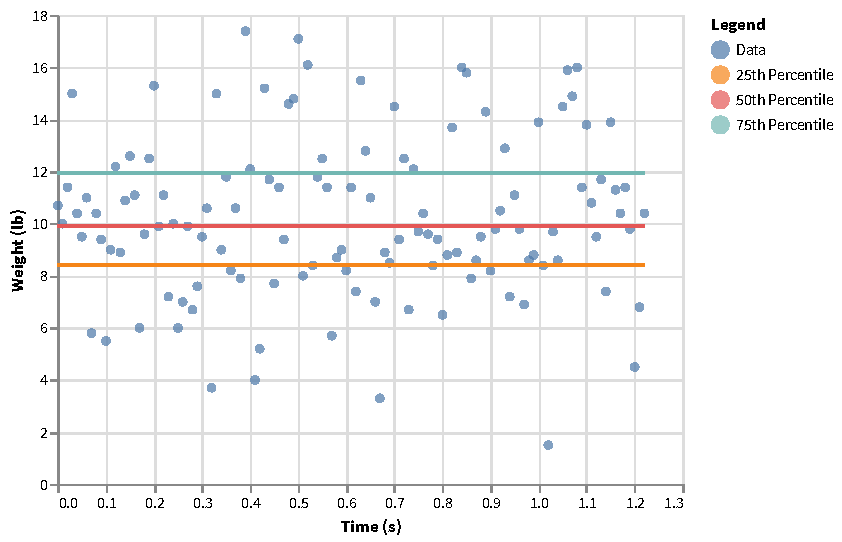
\includegraphics{chart/00-intro/baseline-quartiles.pdf}
    \caption{Quartiles for Baseline Segment}
    \label{figure:00.baseline.quartiles}
\end{figure}
%
\begin{figure}[ht]
    \centering
    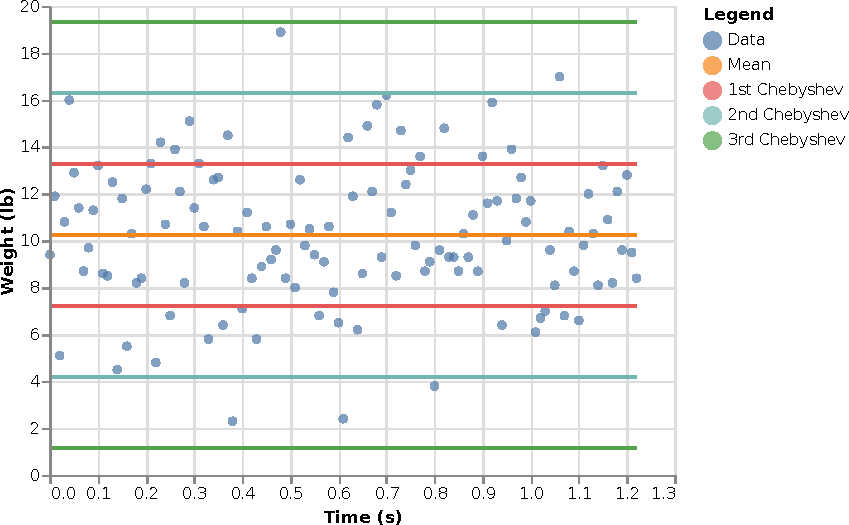
\includegraphics{chart/00-intro/baseline-chebyshev.pdf}
    \caption{Three Chebyshev Intervals for Baseline Segment}
    \label{figure:00.baseline.chebyshev}
\end{figure}
%
\begin{figure}[ht]
    \centering
    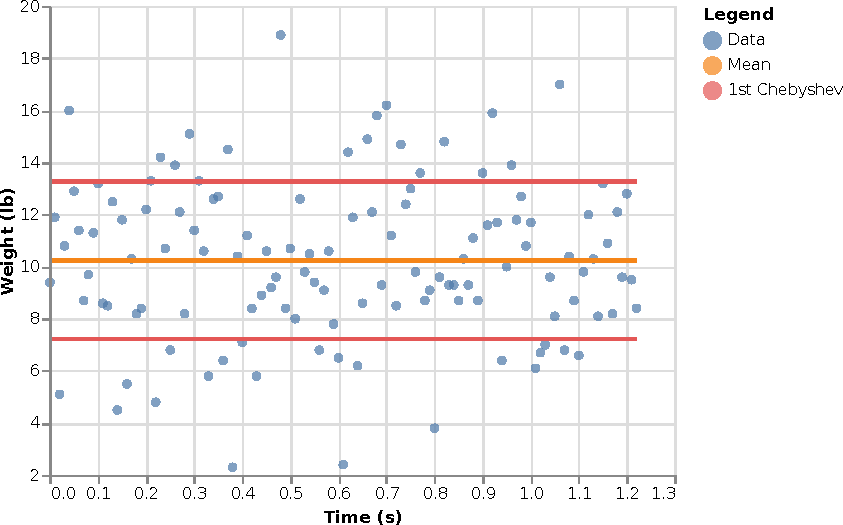
\includegraphics{chart/00-intro/baseline-chebyshev-1.pdf}
    \caption{First Chebyshev Interval for Baseline Segment}
    \label{figure:00.baseline.chebyshev.1}
\end{figure}
%
\begin{figure}[ht]
    \centering
    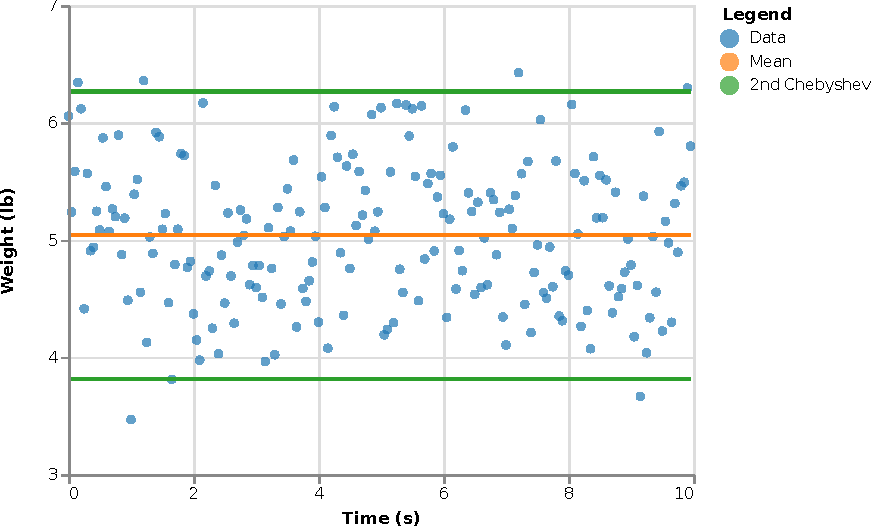
\includegraphics{chart/00-intro/baseline-chebyshev-2.pdf}
    \caption{Second Chebyshev Interval for Baseline Segment}
    \label{figure:00.baseline.chebyshev.2}
\end{figure}
%
\begin{figure}[ht]
    \centering
    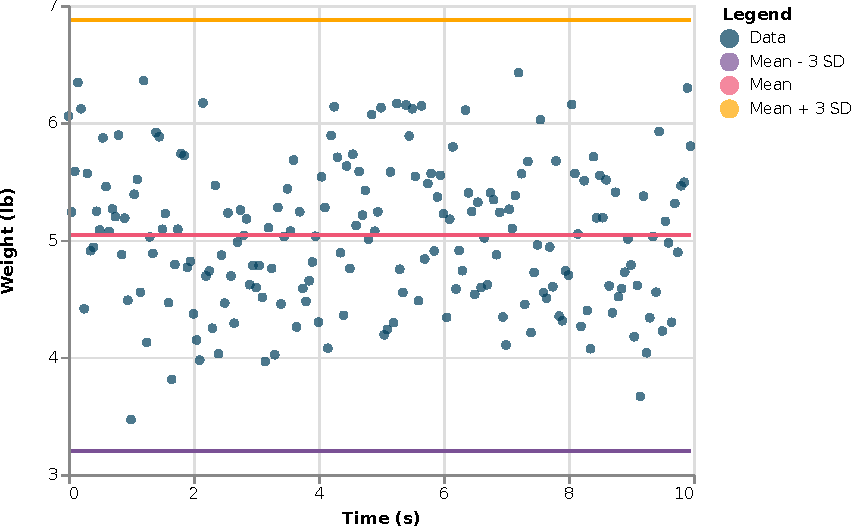
\includegraphics{chart/00-intro/baseline-chebyshev-3.pdf}
    \caption{Third Chebyshev Interval for Baseline Segment}
    \label{figure:00.baseline.chebyshev.3}
\end{figure}
%
\begin{figure}[ht]
    \centering
    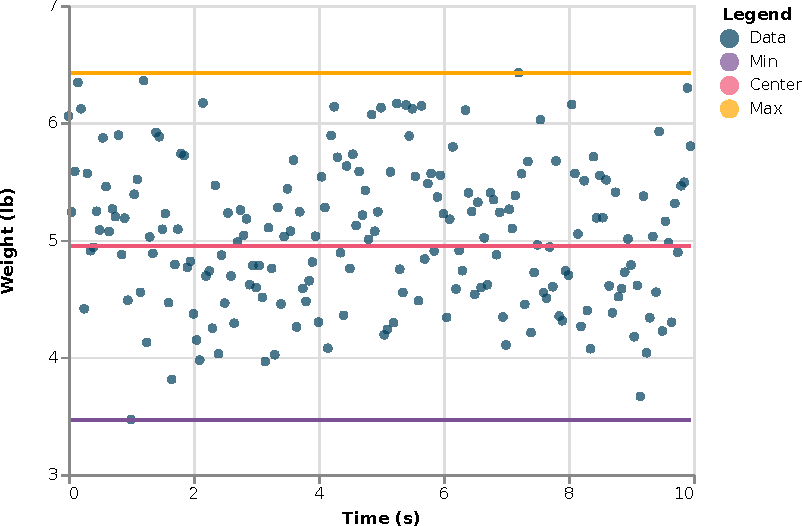
\includegraphics{chart/00-intro/baseline-min-center-max.pdf}
    \caption{Range and Center for Baseline Segment}
    \label{figure:00.baseline.center}
\end{figure}
%
\begin{figure}[ht]
    \centering
    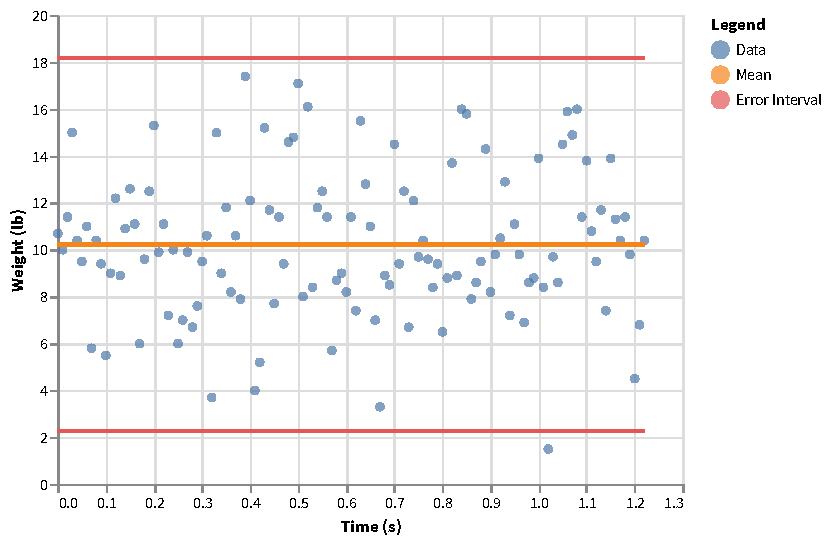
\includegraphics{chart/00-intro/baseline-error-interval.pdf}
    \caption{Error Interval for Baseline Segment}
    \label{figure:00.baseline.interval}
\end{figure}
%
\begin{figure}[ht]
    \centering
    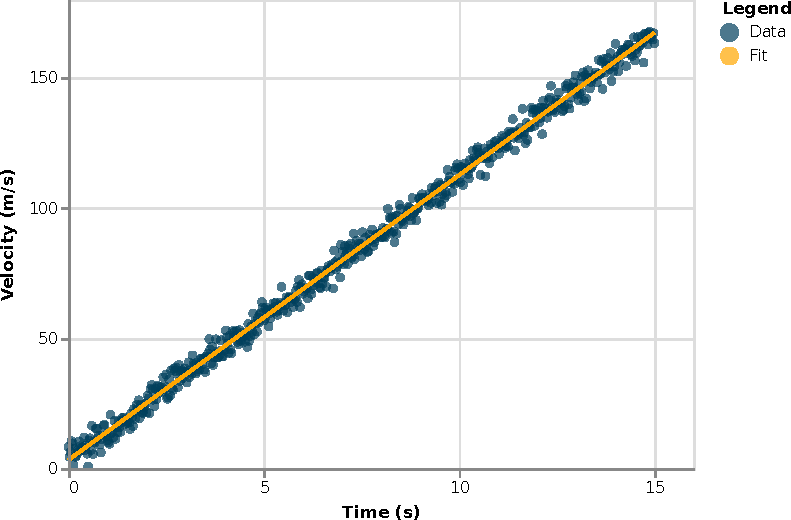
\includegraphics{chart/00-intro/velocity-fit.pdf}
    \caption{Velocity Data and Best Fit}
    \label{figure:00.velocity.fit}
\end{figure}
%
